\documentclass[aspectratio=169,x11names]{beamer}
\usetheme{Pittsburgh}
\usepackage{xcolor}
\usepackage[utf8]{inputenc}
\usepackage[german]{babel}
\usepackage{amsmath}
\usepackage{amsfonts}
\usepackage{amssymb}
\usepackage{graphicx}
\usepackage{multicol}
\usepackage{wrapfig}
\usepackage{hyperref}
\usepackage{tikz}

\usetikzlibrary{shapes,arrows,chains}

\author{Jonas Betzendahl}
\title{Algorithmen und Du}

\beamertemplatenavigationsymbolsempty 

%src: https://tex.stackexchange.com/questions/34921/how-to-overlap-images-in-a-beamer-slide
\def\Put(#1,#2)#3{\leavevmode\makebox(0,0){\put(#1,#2){#3}}}

\begin{document}

%------------------------------------------------------------------------------------
\section{Introduction}

\begin{frame}
\begin{center}
\vfill
\huge Algorithmen und Du
\normalsize 
\smallskip
\smallskip

Warum Künstliche Intelligenz nie politisch neutral sein kann
\bigskip\bigskip

\large Jonas Betzendahl, M.Sc.
\bigskip\bigskip

\href{https://twitter.com/lambdatotoro}{
\includegraphics[scale=0.125]{images/twitter_logo.png}}
\href{https://chaos.social/@lambdatotoro}{\includegraphics[scale=0.125]{images/mastodon_logo.png}}
\href{https://github.com/jbetzend}{
\includegraphics[scale=0.125]{images/github_logo.png}}
\href{https://whispeer.de/en/user/jbetzend}{
\includegraphics[scale=0.125]{images/whispeer_logo.png}}

\texttt{@lambdaTotoro (@chaos.social)}
\end{center}
\end{frame}

%------------------------------------------------------------------------------------


\begin{frame}
\begin{center}
\huge
Künstliche Intelligenz
\bigskip

\large
The hype is real\dots
\end{center}
\end{frame}

\begin{frame}
\frametitle{Menschen sind \emph{sehr} fehlbar...}
\begin{minipage}{0.5\textwidth}
\begin{center}
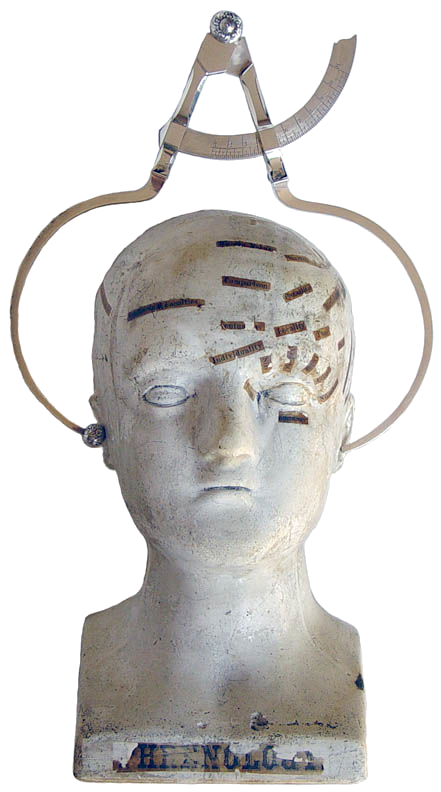
\includegraphics[keepaspectratio, height=0.75\textheight]{images/calipers_transparent}
\end{center}
\end{minipage}\begin{minipage}{0.5\textwidth}
\begin{center}
\pause

\includegraphics[keepaspectratio, height=0.75\textheight]{images/human_bias}
\end{center}
\end{minipage}
\end{frame}

\begin{frame}
\frametitle{...und \emph{sehr} langsam!}
\begin{center}
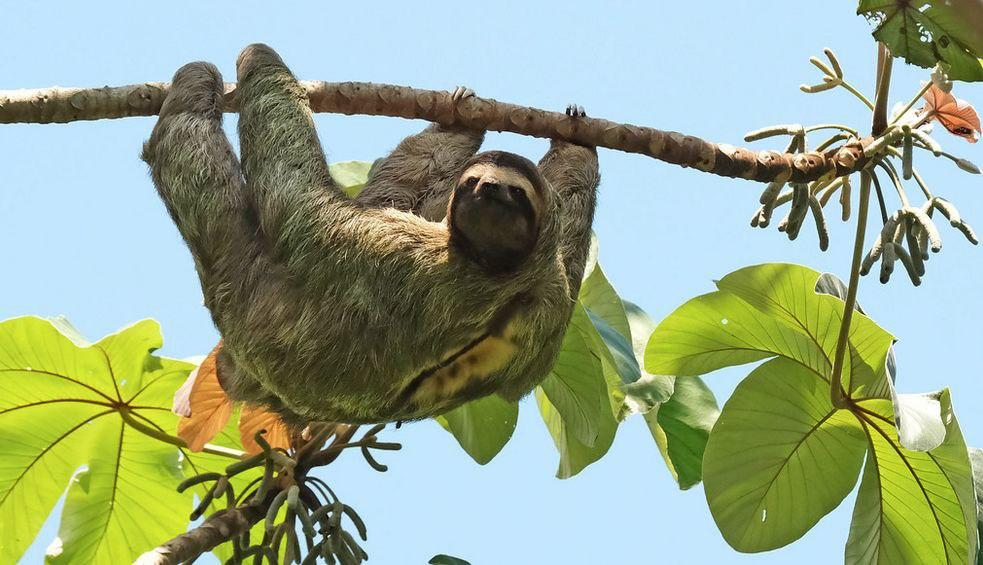
\includegraphics[height=0.75\textheight, keepaspectratio]{images/sloth}
\end{center}
\end{frame}

\begin{frame}
\begin{center}
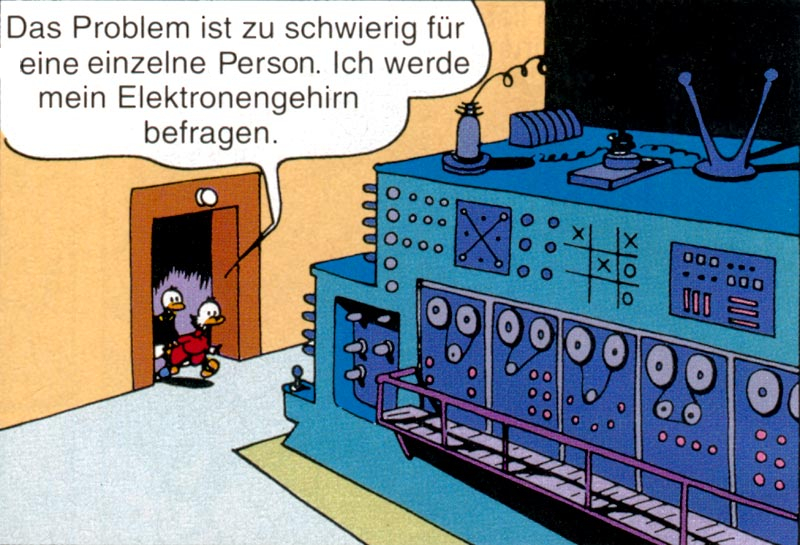
\includegraphics[keepaspectratio, height=0.85\textheight]{images/elektronengehirn}
\end{center}
\pause
\Put(30,400){
\includegraphics[scale=0.4, angle=5]{images/ki_lufthansa}}
\pause
\Put(20,240){
\includegraphics[scale=0.25, angle=25]{images/gema_ki_klein}}
\pause
\Put(10,350){
\includegraphics[scale=0.4, angle=-15]{images/ki_suicide}}
\pause
\Put(10,125){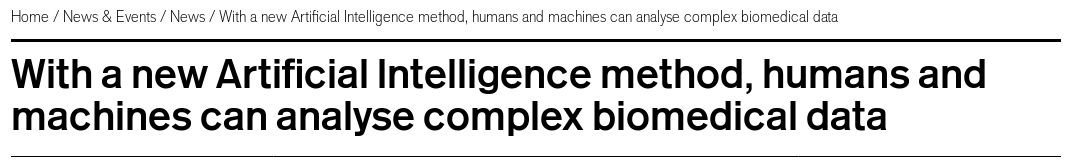
\includegraphics[scale=0.3, angle=-4]{images/ki_medicine}}
\pause
\Put(80,250){
\includegraphics[scale=0.35, angle=10]{images/ki_law}}
\pause
\Put(40,250){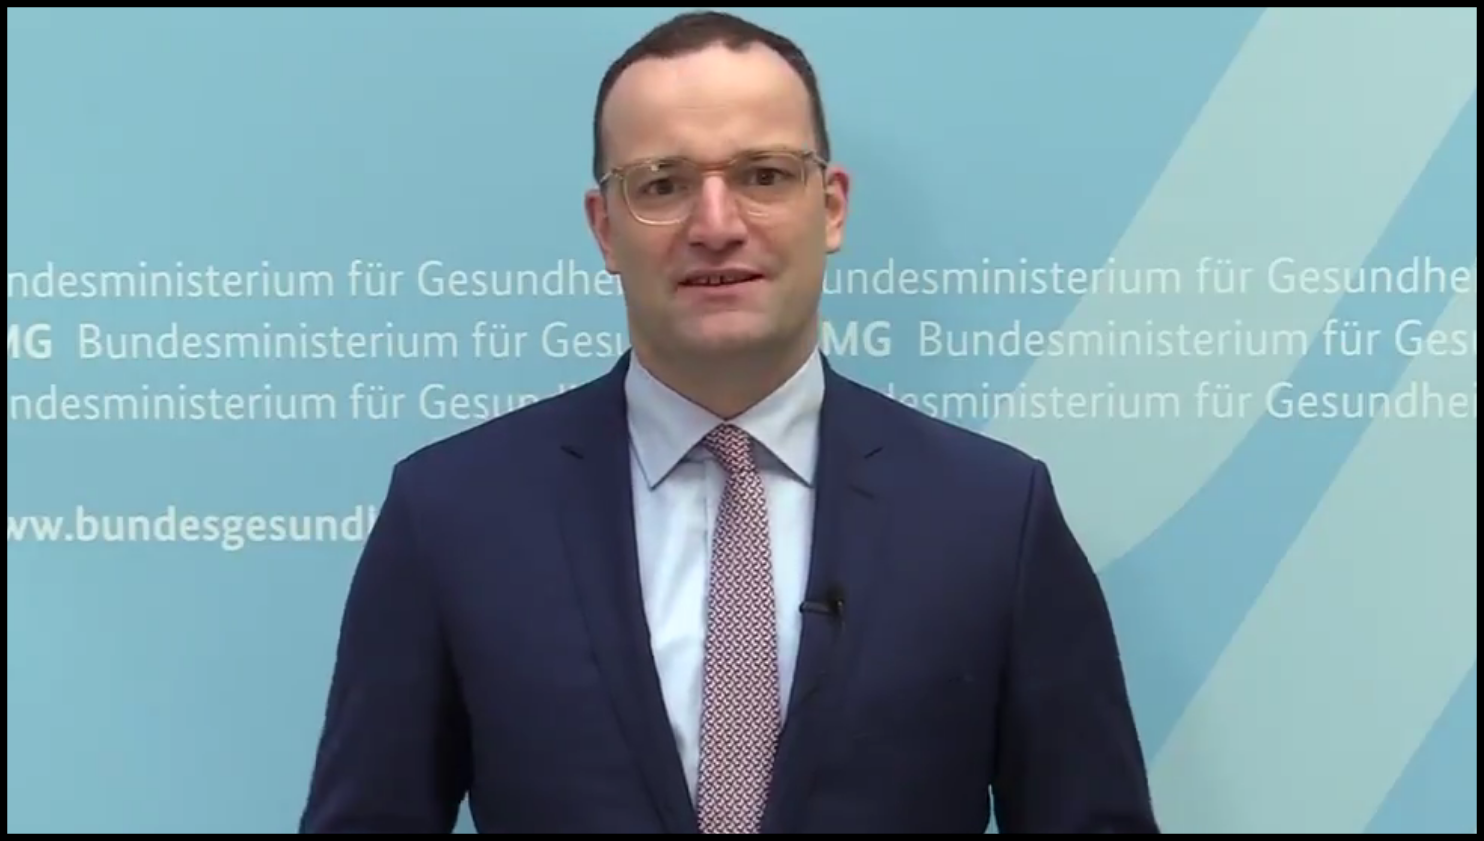
\includegraphics[scale=0.8]{images/spahn}}
\end{frame}

%\begin{frame}
%\frametitle{Bonusrunde!}
%\begin{center}
%\large
%Science-Slam-ception!
%
%\huge
%\emph{Blockchains}
%\bigskip
%
%\large
%Macht eine Blockchain für mich, meine Firma\\ oder meine Organisation Sinn?
%\pause
%\bigskip\bigskip\bigskip
%
%\Huge
%
\includegraphics[scale=0.65]{images/pointing.png} \textcolor{red}{\textbf{\textit{Nein!}}} 
\includegraphics[scale=0.65]{images/pointing2.png}
%\end{center}
%\end{frame}

%------------------------------------------------------------------------------------

\section{How it works and weaknesses}

\begin{frame}
\begin{center}
\huge
Algorithmen \&\\
Maschinelles Lernen
\bigskip

\large
Was ist das? Wie geht das?\\ Und was sind die Probleme?
\end{center}
\end{frame}

\begin{frame}
\frametitle{Algorithmen}
\begin{center}

\includegraphics[height=0.7\textheight, keepaspectratio]{images/recipe}

Alltäglicher als vielleicht gedacht\dots
\end{center}
\end{frame}


\begin{frame}
\frametitle{Maschinelles Lernen}
\begin{center}

\includegraphics[height=0.8\textheight, keepaspectratio]{images/funnel}
\end{center}
\end{frame}

\begin{frame}[fragile]
\frametitle{Beeindruckende Mathematik}

\begin{minipage}{0.52\textwidth}
\begin{center}
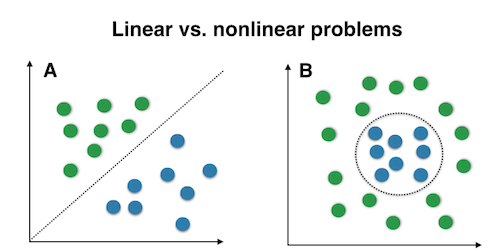
\includegraphics[scale=0.3]{images/linear_nonlinear.png} 
\end{center}
\end{minipage}\begin{minipage}{0.35\textwidth}
$$y_k = \varphi\left(\sum_{j=0}^m w_{kj}x_j\right)$$
\end{minipage}

\small
\begin{minipage}{0.47\textwidth}
$$\Delta w_{ij}=-\eta \frac{\partial E}{\partial w_{ij}} = -\eta o_i \delta_j$$
$$\lambda(x) = C(t-x)^2$$
$$r_i \dot{y_i} = -y_i \sum_{j=1}^n w_{ji}\sigma\left(y_j - \Theta_j\right) * I_i(t)$$
\end{minipage}\begin{minipage}{0.47\textwidth}
\begin{center}
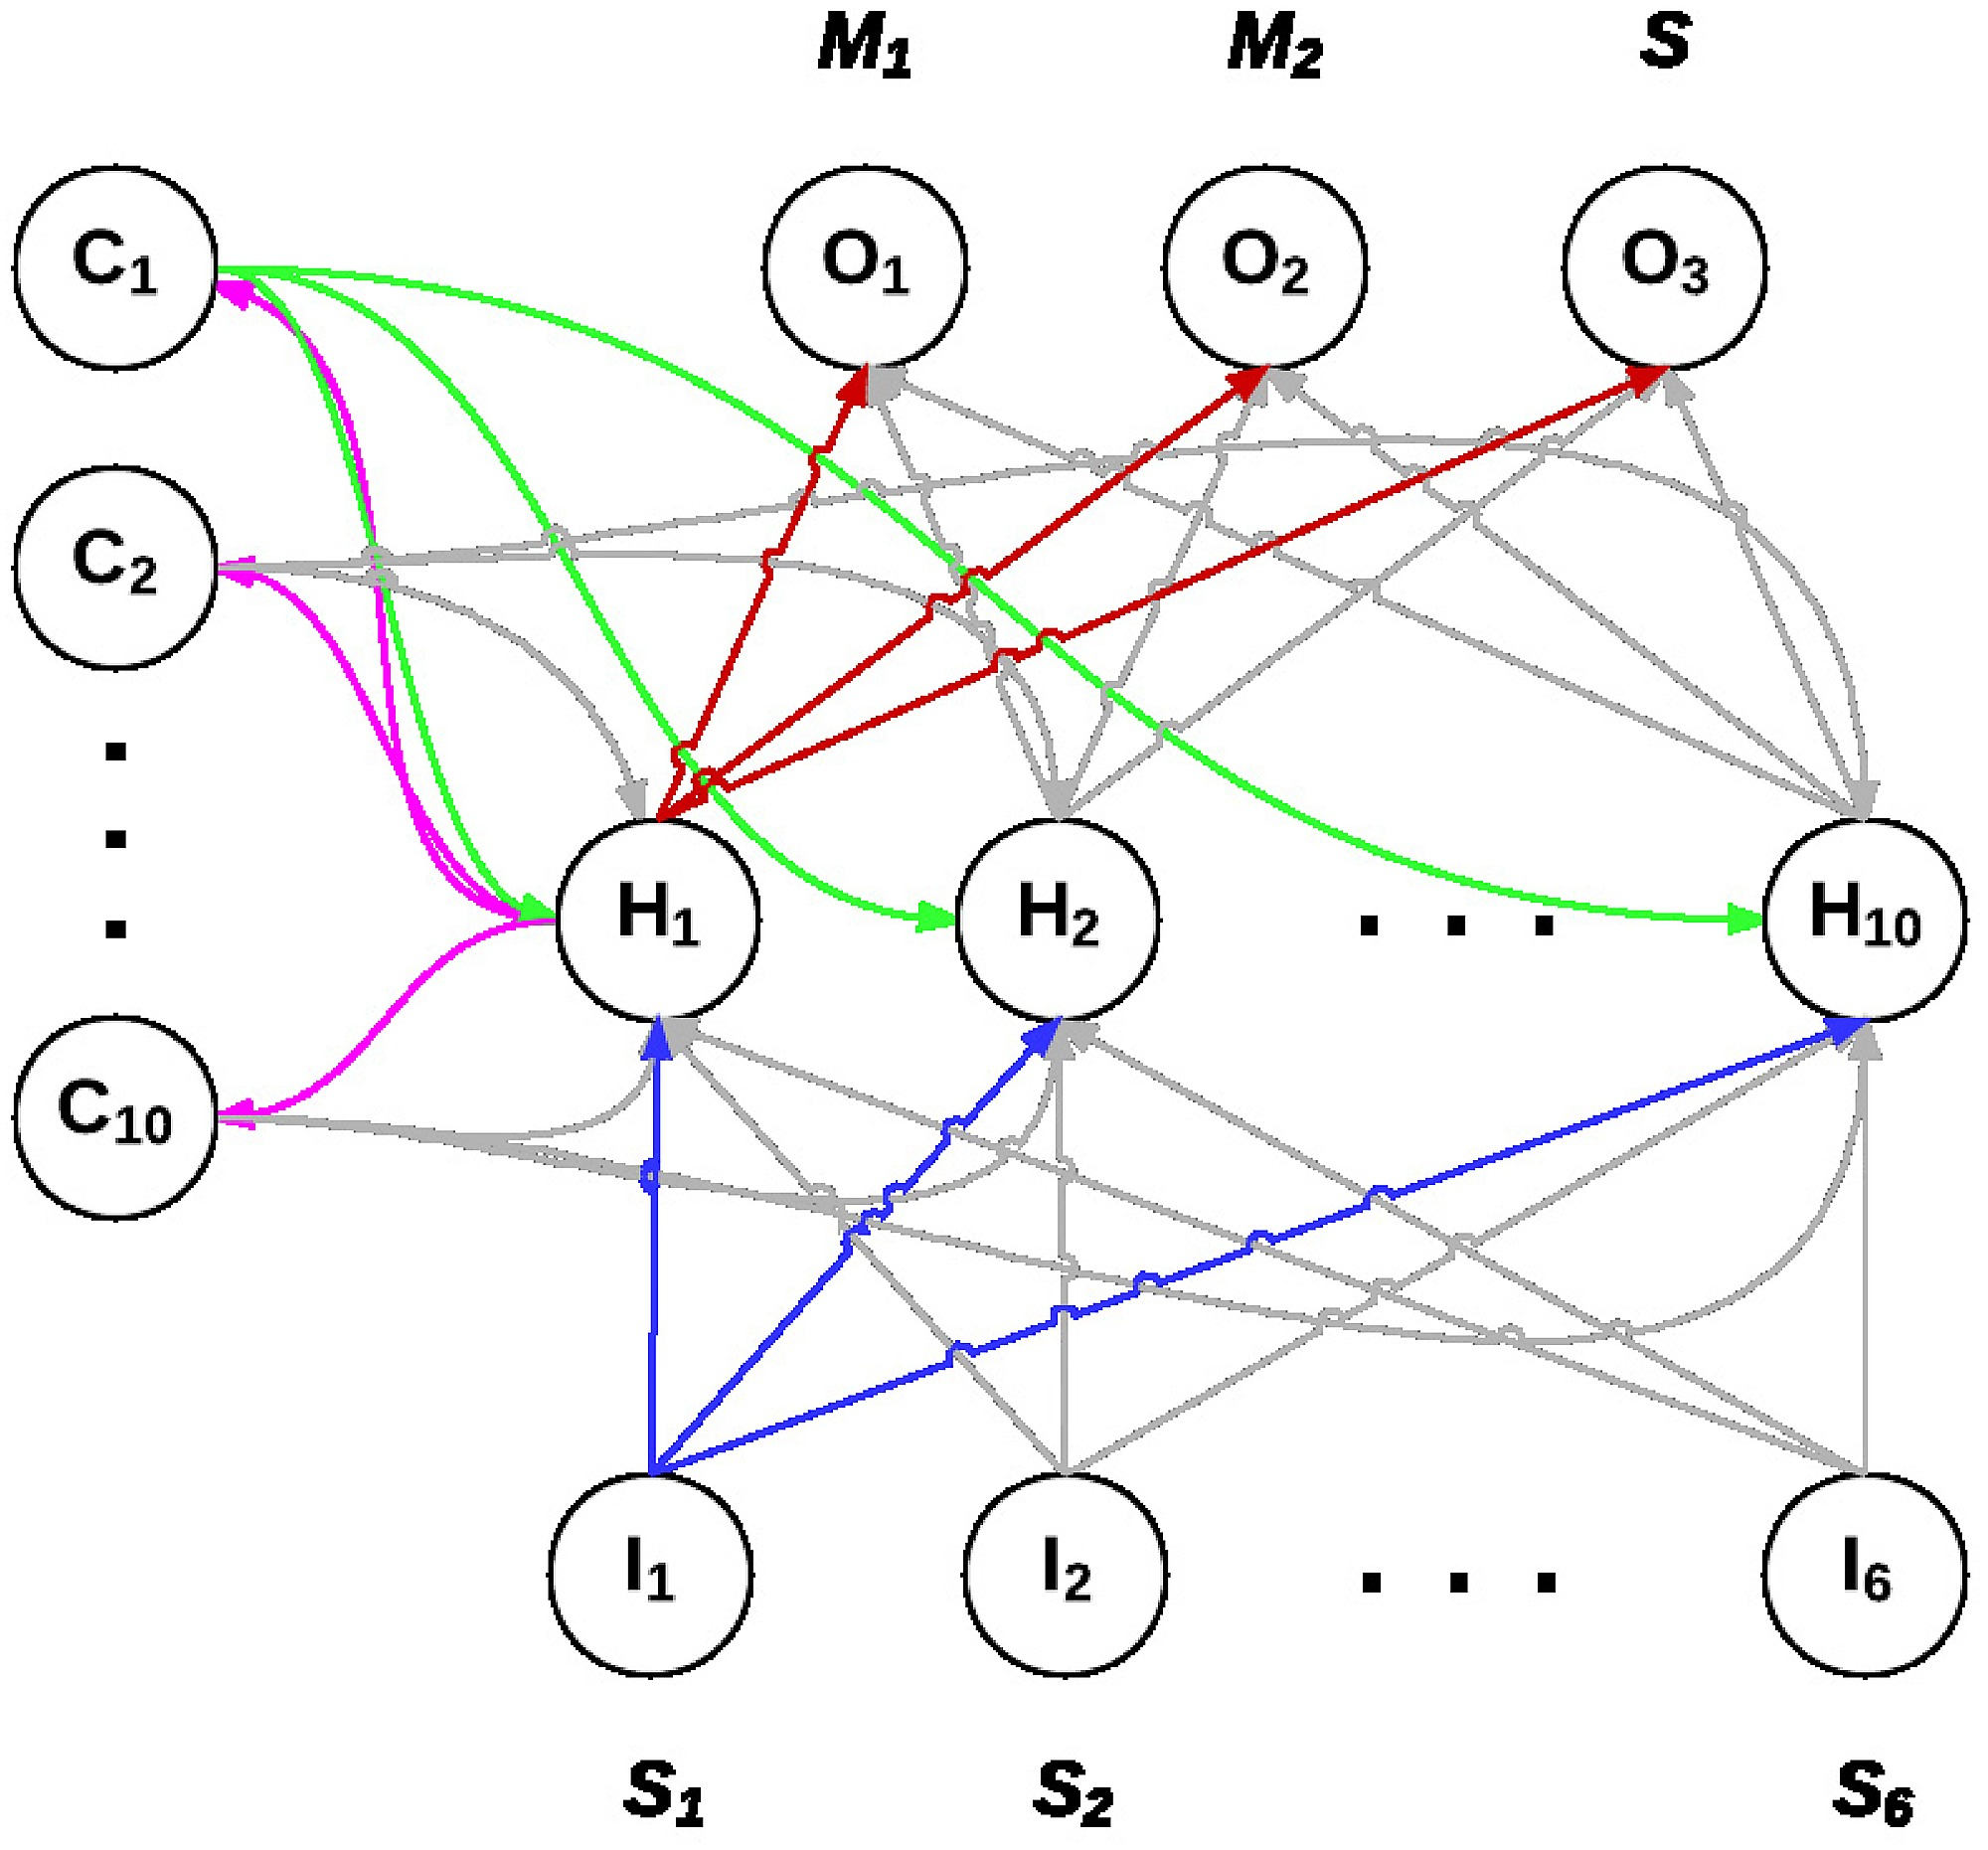
\includegraphics[scale=0.35]{images/recursive.jpg} 
\end{center}
\end{minipage}
\end{frame}

\begin{frame}
\frametitle{Limitierungen}

Trotz allen Buzzwords, immer fragen: \dots \bigskip

\begin{itemize}
\pause\item Auf welchen Daten lernen wir?\\

\pause\item Wer bestimmt worauf optimiert wird?\\

\pause\item Was sind die Folgen? Selbsterfüllende Prophezeihung?\\
\end{itemize}

\pause\bigskip

Und immer daran denken: \dots
\begin{itemize}
\item ML gibt immer nur ein \emph{Was}, niemals ein \emph{Warum}!
\end{itemize}
\end{frame}

%------------------------------------------------------------------------------------

\section{Surely nobody would be this stupid?}

\begin{frame}
\begin{center}
\huge
KI in der freien Wildbahn
\bigskip

\large
Leider nicht nur theoretisch problematisch\dots
\end{center}
\end{frame}

\begin{frame}
\frametitle{Erkennung von Panzern}
\begin{center}
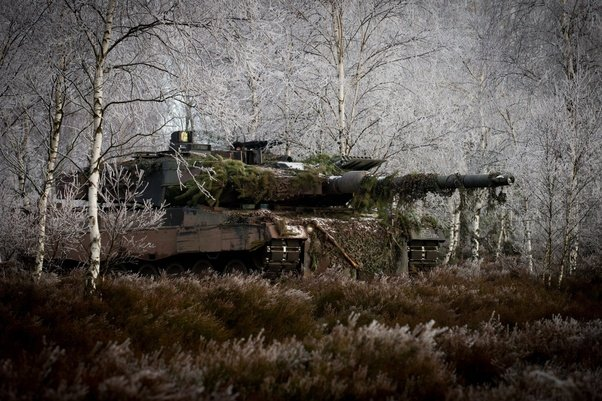
\includegraphics[height=0.7\textheight, keepaspectratio]{images/tank}

Der vielleicht spektakulärste Fehlschlag des Feldes!
\pause
\Put(-275,220){
\includegraphics[scale=0.45, angle=10]{images/princess_bride.jpg} }
\end{center}
\end{frame}

\begin{frame}
\frametitle{Konsequenzen am Arbeitsmarkt}
\begin{minipage}{.5\textwidth}
\begin{center}
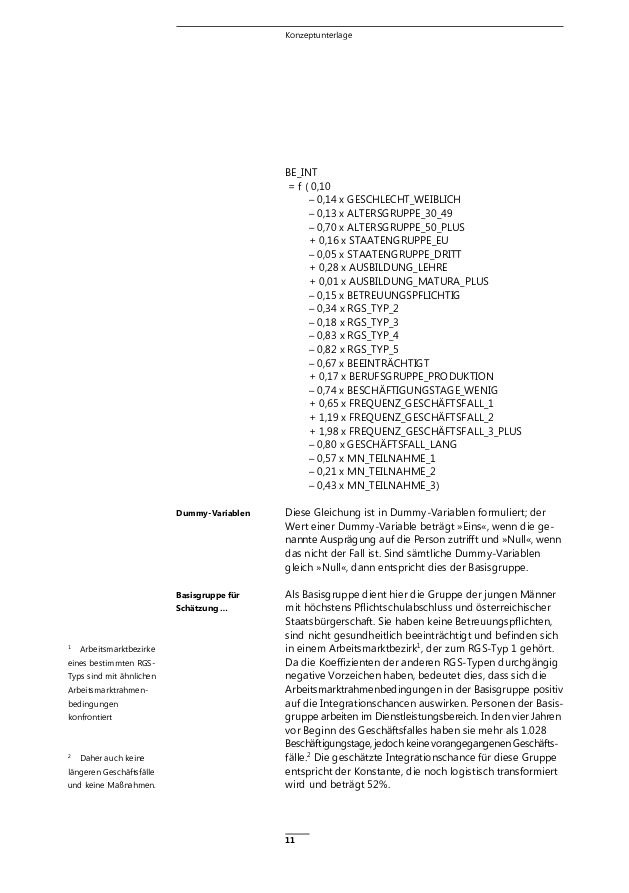
\includegraphics[height=0.75\textheight, keepaspectratio]{images/negativfaktor}
\end{center}
\end{minipage}\begin{minipage}{.5\textwidth}
\begin{center}
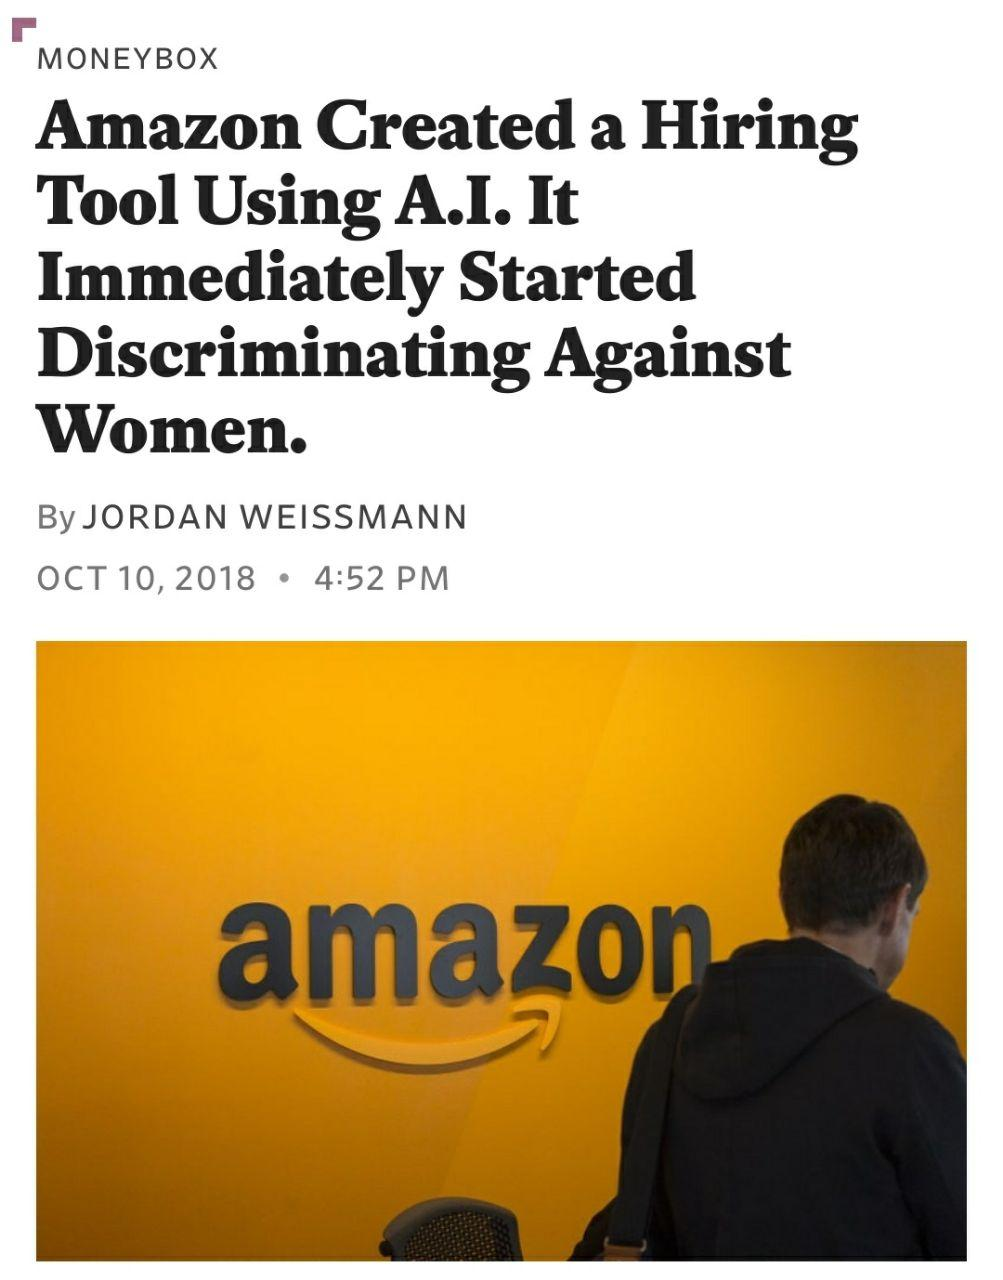
\includegraphics[height=0.75\textheight, keepaspectratio]{images/amazon_hiring}
\end{center}
\end{minipage}

\pause
\Put(70,250){
\includegraphics[scale=1.8, angle=-10]{images/any_of_this} }
\end{frame}

\begin{frame}
\frametitle{Finanzielle Konsequenzen}
\begin{center}

\includegraphics[scale=0.3]{images/apple_0}
\end{center}

\pause
\Put(70,275){
\includegraphics[scale=0.3, angle=-10]{images/apple_1}}
\pause
\Put(50,250){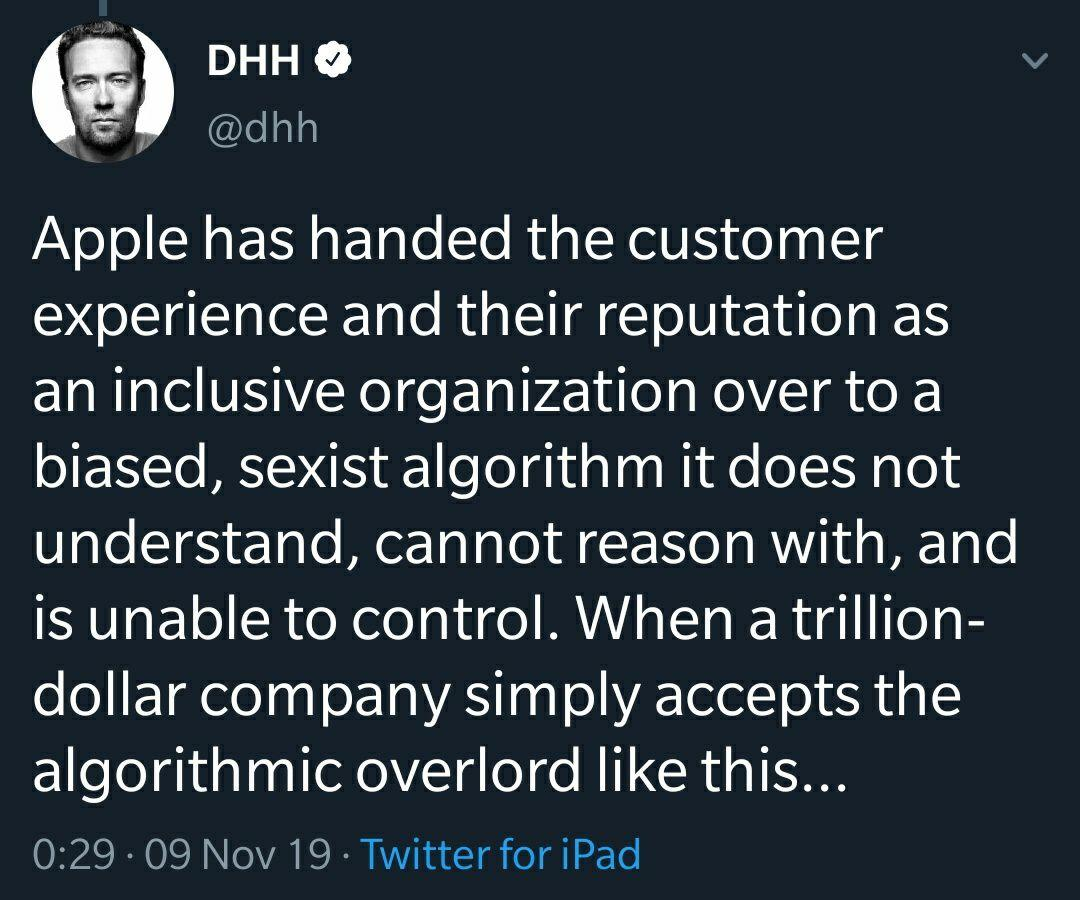
\includegraphics[scale=0.3, angle=10]{images/apple_2}}

\pause
\Put(180,170){
\includegraphics[scale=1.75, angle=30]{images/manshrug}}

\end{frame}

\begin{frame}
\frametitle{Erkennen von sexueller Orientierung?}
\begin{minipage}{.6\textwidth}
\begin{center}
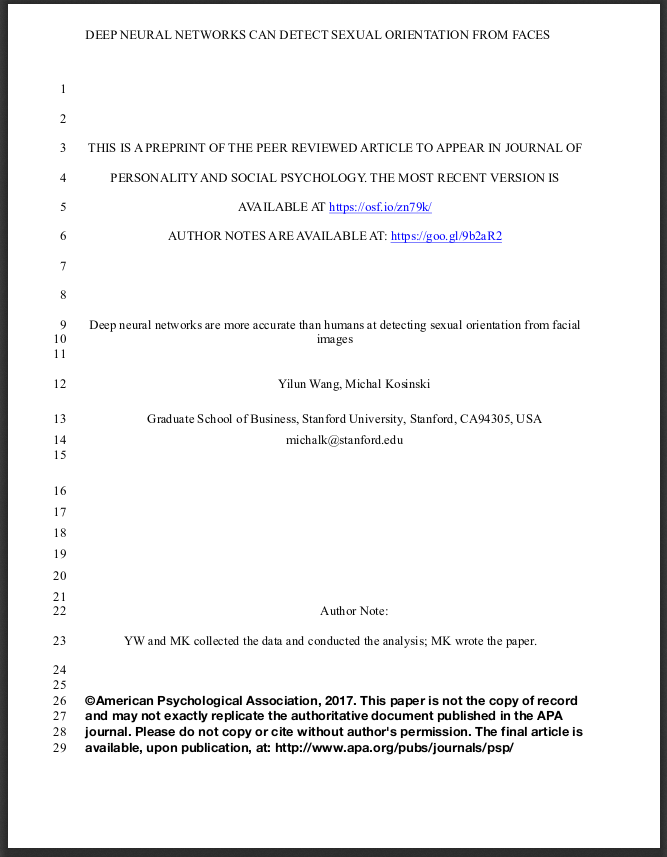
\includegraphics[height=0.75\textheight, keepaspectratio]{images/paper_orientation}
\end{center}
\end{minipage}\hspace*{-25pt}\begin{minipage}{.4\textwidth}
\begin{center}
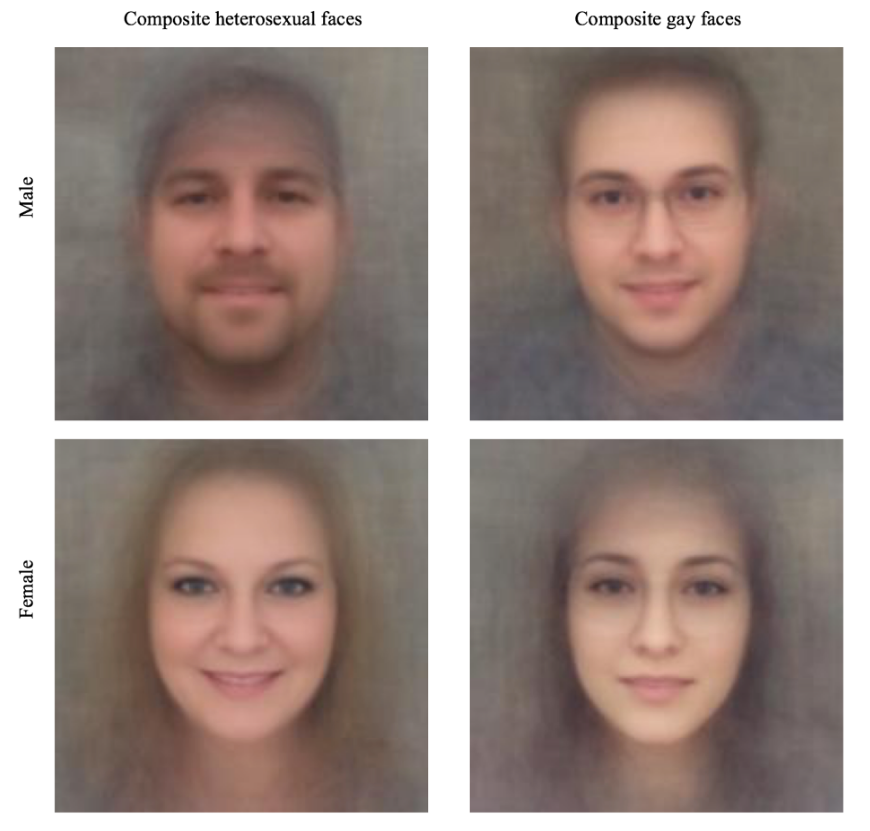
\includegraphics[width=0.99\textwidth, keepaspectratio]{images/composite_faces}
\end{center}
\end{minipage}

\pause
\Put(50,200){
\includegraphics[scale=0.45, angle=15]{images/princess_bride.jpg} }
\pause
\Put(50,250){
\includegraphics[scale=0.225, angle=-15]{images/goldblum} }
\end{frame}

\begin{frame}
\frametitle{``Phrenology as a Service''}
\begin{center}
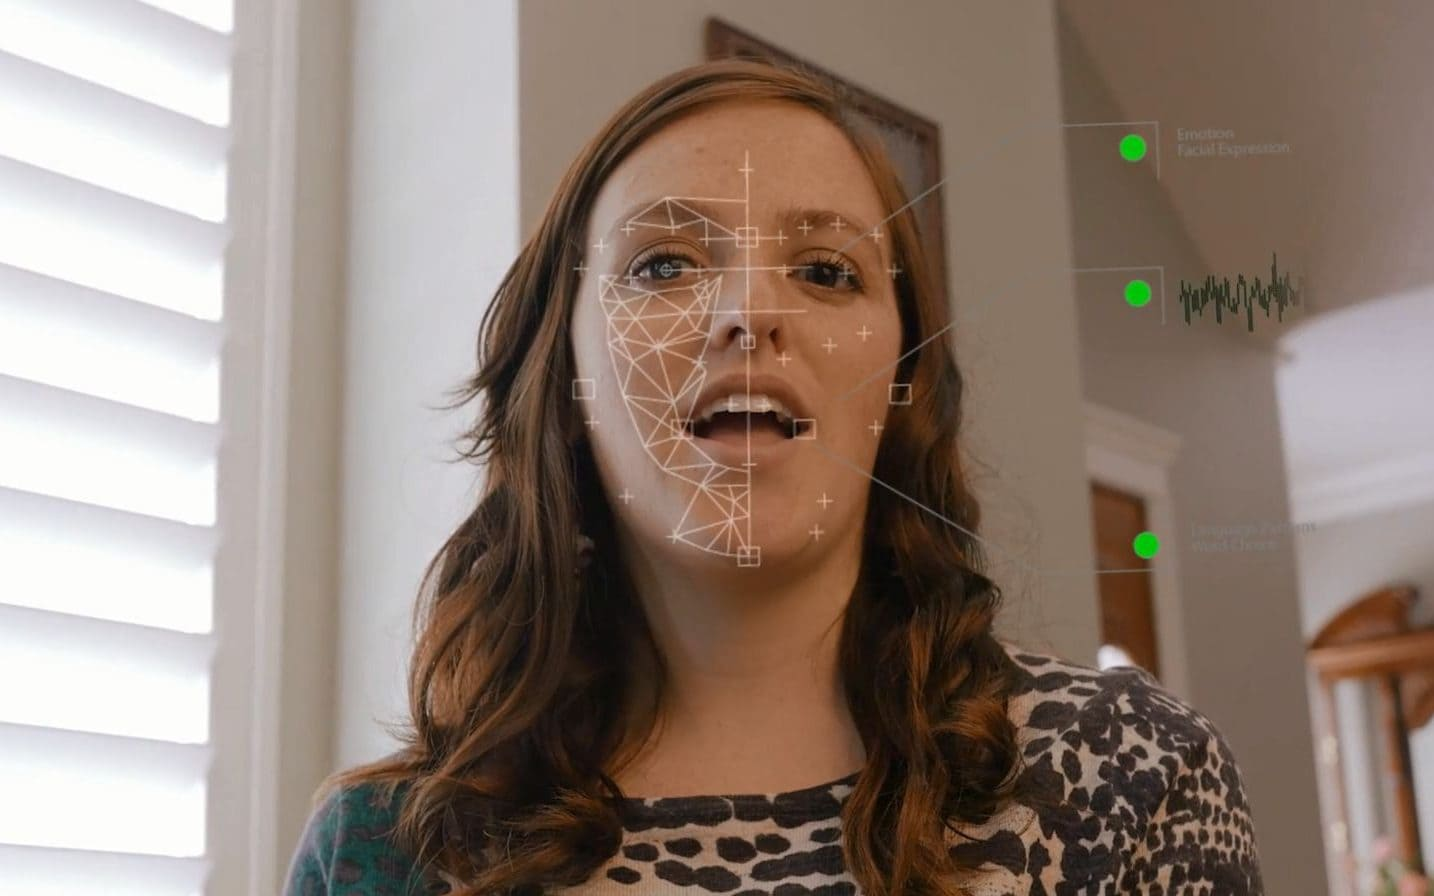
\includegraphics[keepaspectratio, height=0.7\textheight]{images/hirevue}

\large
Gesichtsanalyse im Bewerbungsgespräch
\end{center}
\pause
\Put(135,275){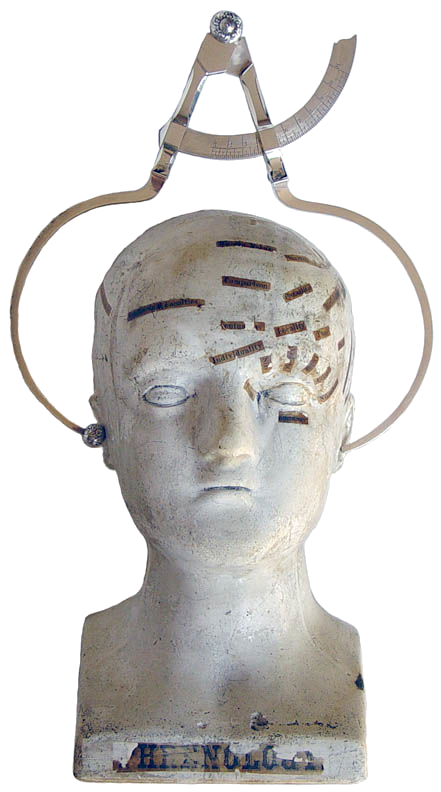
\includegraphics[scale=0.3]{images/calipers_transparent}}
\end{frame}

\begin{frame}
\begin{center}

\includegraphics[keepaspectratio, height=0.85\textheight]{images/thomas}
\end{center}
\end{frame}

%------------------------------------------------------------------------------------

\section{What to do about it?}

\begin{frame}
\begin{center}
\huge
Was tun wir dagegen?

\large
take-home messages
\normalsize
\end{center}
\bigskip

Jedes Mal wenn \glqq Künstliche Intelligenz\grqq\ oder \glqq Maschinelles Lernen\grqq\ aufkommen:
\medskip

\begin{itemize}
\item \emph{Woher} wird gelernt? Welches \emph{Datenset} wird benutzt?
\item \emph{Was} wird gelernt? Worauf wird \emph{optimiert}?
\item Was sind die \emph{Folgen} von diesen Entscheidungen?
\item Haben wir eine Möglichkeit, \emph{Menschen} entscheiden zu lassen?
\end{itemize}

\pause\bigskip\bigskip
\begin{center}
\large
skeptisch bleiben!
\end{center}
\Put(265,45){
\includegraphics[scale=0.5, keepaspectratio]{images/thinking_emoji}}
\end{frame}

%------------------------------------------------------------------------------------

\begin{frame}
\frametitle{Quellen:}
\scriptsize
\begin{itemize}
\item Diskriminierung b. Wohnungssuche ``Hanna und Ismail'', Köppen et al.  2017\\
\url{https://www.hanna-und-ismail.de/}

\item ``Amazon Created a Hiring Tool Using A.I. It Immediately Started Discriminating Against Women.'', Weissmann, 2018\\ \url{https://slate.com/business/2018/10/amazon-artificial-intelligence-hiring-discrimination-women.html}

\item ``Machine Bias'', Angwin et al., ProPublica, 2016\\ \url{https://www.propublica.org/article/machine-bias-risk-assessments-in-criminal-sentencing}

\item ``Deep Neural Networks Are More Accurate Than Humans at Detecting Sexual Orientation From Facial Images'', Kosinski et al., 2018\\ \url{https://www.gsb.stanford.edu/faculty-research/publications/deep-neural-networks-are-more-accurate-humans-detecting-sexual}

\item ``Negativfaktor Frau'', Ingrid Brodnig, 2018 \\ \url{www.profil.at/meinung/ingrid-brodnig-negativfaktor-frau-10422551}

\item ``AI used for first time in job interviews in UK to find best applicants'', The Telegraph, 2019-09-27 \\ \url{https://www.telegraph.co.uk/news/2019/09/27/ai-facial-recognition-used-first-time-job-interviews-uk-find/}

\end{itemize}
\end{frame}
\end{document}

